%!TEX root = TFG.tex

\chapter{Resultados} \label{chap:result}

Una vez entrenados todos los algoritmos con sus mejores hiperparámetros, se obtienen los resultados de los modelos de clasificación, que se pueden ver en la Fig. \ref{fig:comp_accur}; y también los resultados que aportan los modelos de detección de anomalías, presentados en la Tabla \ref{tab:anomaly_results}.

Para analizar todos estos modelos se hará uso de diversas métricas, como las que se presentan entre las fórmulas \ref{eq:accur} y \ref{eq:tnr}. Para obtener estas métricas es necesario hacer uso de matrices de confusión.

Una matriz de confusión es una tabla que evalúa los resultados de un modelo Machine Learning orientado a la clasificación. En este tipo de tablas se enfrentan valores bien predichos y mal predichos observando las etiquetas reales y las predichas por los datos. Un ejemplo de matriz de confusión se puede ver a continuación en la Tabla \ref{tab:ex_confusion_matrix}. Con este tipo de herramientas en sencillo ver los aciertos y fallos de un modelo. Esta herramienta también se puede generalizar a clasificación multiclase, que ha sido el uso en este trabajo.

\begin{table}
    \centering
    \begin{tabular}{@{}cc cc@{}}
        \multicolumn{1}{c}{} &\multicolumn{1}{c}{} &\multicolumn{2}{c}{Valor predicho} \\ 
        \cmidrule(lr){3-4}
        \multicolumn{1}{c}{} & 
        \multicolumn{1}{c}{} & 
        \multicolumn{1}{c}{Sí} & 
        \multicolumn{1}{c}{No} \\ 
        \cline{2-4}
        \multirow[c]{2}{*}{\rotatebox[origin=tr]{90}{$\underset{\text{real}}{\text{Valor}}$}}
        & Sí  & Verdadero positivo ($TP$) & Falso positivo ($FP$) \\
        & No  & Falso negativo ($FN$) & Verdadero negativo ($TN$) \\ 
        \cline{2-4}
    \end{tabular}
    \caption{Ejemplo de matriz de confusión}
    \label{tab:ex_confusion_matrix}
\end{table}

Con una matriz de confusión es posible obtener las distintas métricas que sirven para comparar los modelos de Machine Learning como Accuracy, Recall, True Negative Rate (TNR), $f$-score.

\begin{multicols}{2}
\begin{equation}
    Accuracy = \frac{TP + TN}{TP + FP + FN + TN}
    \label{eq:accur}
\end{equation}
\begin{equation}
    Recall = \frac{TP}{TP + FN}
    \label{eq:recall}
\end{equation}
\begin{equation}
    f-score = \frac{2 \cdot TP}{2 \cdot TP + FP + FN}
\end{equation}
\begin{equation}
    TNR = \frac{TN}{TN + FP}
    \label{eq:tnr}
\end{equation}
\end{multicols}

Analizando en primer lugar los modelos de clasificación, se puede ver en la figura anteriormente mencionada, Fig. \ref{fig:comp_accur}, que los modelos que presentan mejores resultados son los que se basan en árboles de decisión, que son el propio algoritmo de árboles de decisión y random forest. Otra forma de ver estos resultados es mediante las matrices de confusión que genera cada algoritmo.

\begin{figure}[htpb!]
    \centering
    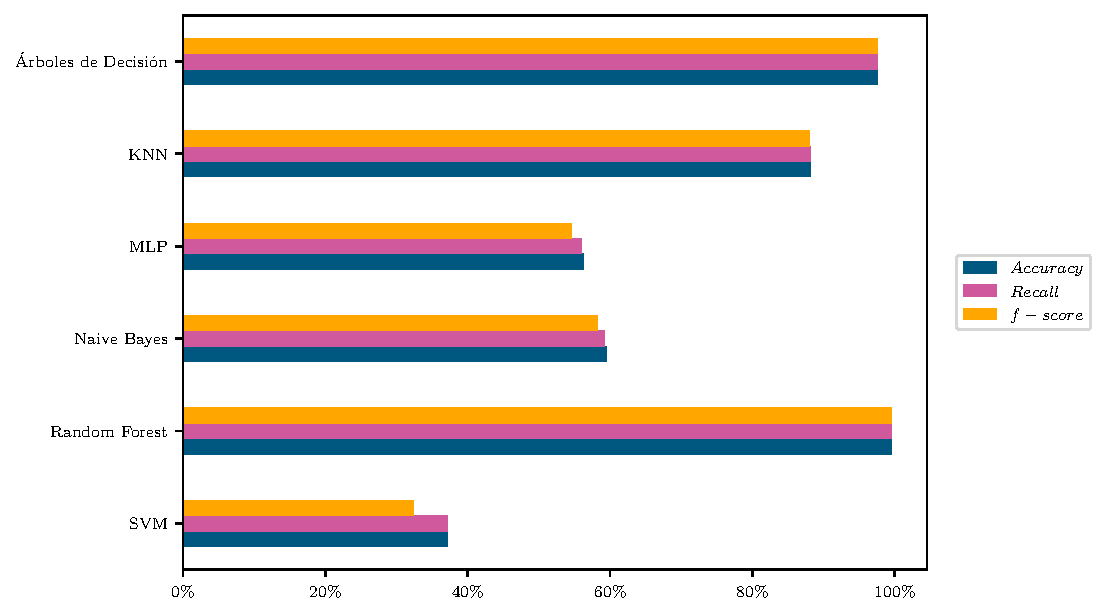
\includegraphics[width=0.6\textwidth]{../Python/plots/parallel/model_results}
    \caption{Comparativa de resultados entre modelos de clasificación}
    \label{fig:comp_accur}
\end{figure}

Es fácil ver en la Fig. \ref{fig:confusion_matrices_parallel} que los modelos basados en árboles aciertan prácticamente en la totalidad de las ocasiones, en particular, el algoritmo de Random Forest es el que mejores resultados consigue con aproximadamente 99.5\% en todas las métricas analizadas, seguido de cerca por Árboles de Decisión con aproximadamente 97.6\% en todas las métricas.


\begin{figure}[htpb!]
    \centering
    \begin{tabular}{ccc}
        \subfloat{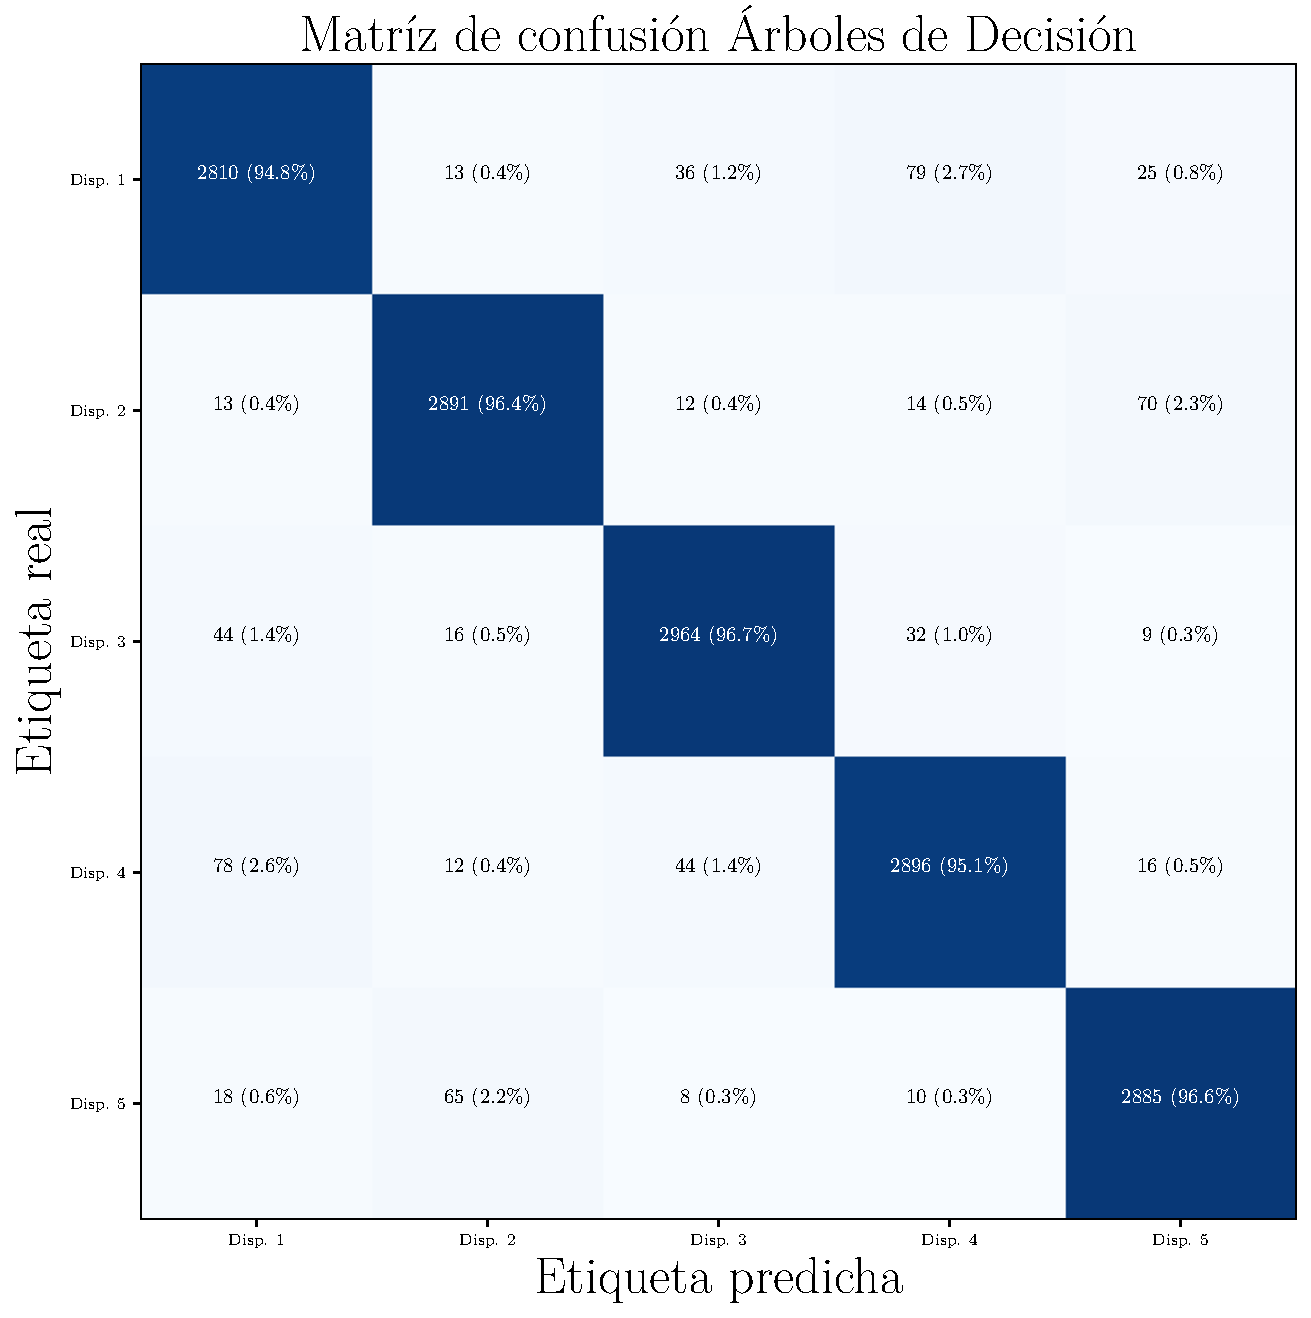
\includegraphics[width=0.4\textwidth]{../Python/plots/parallel/decision_tree_matrix}} & \subfloat{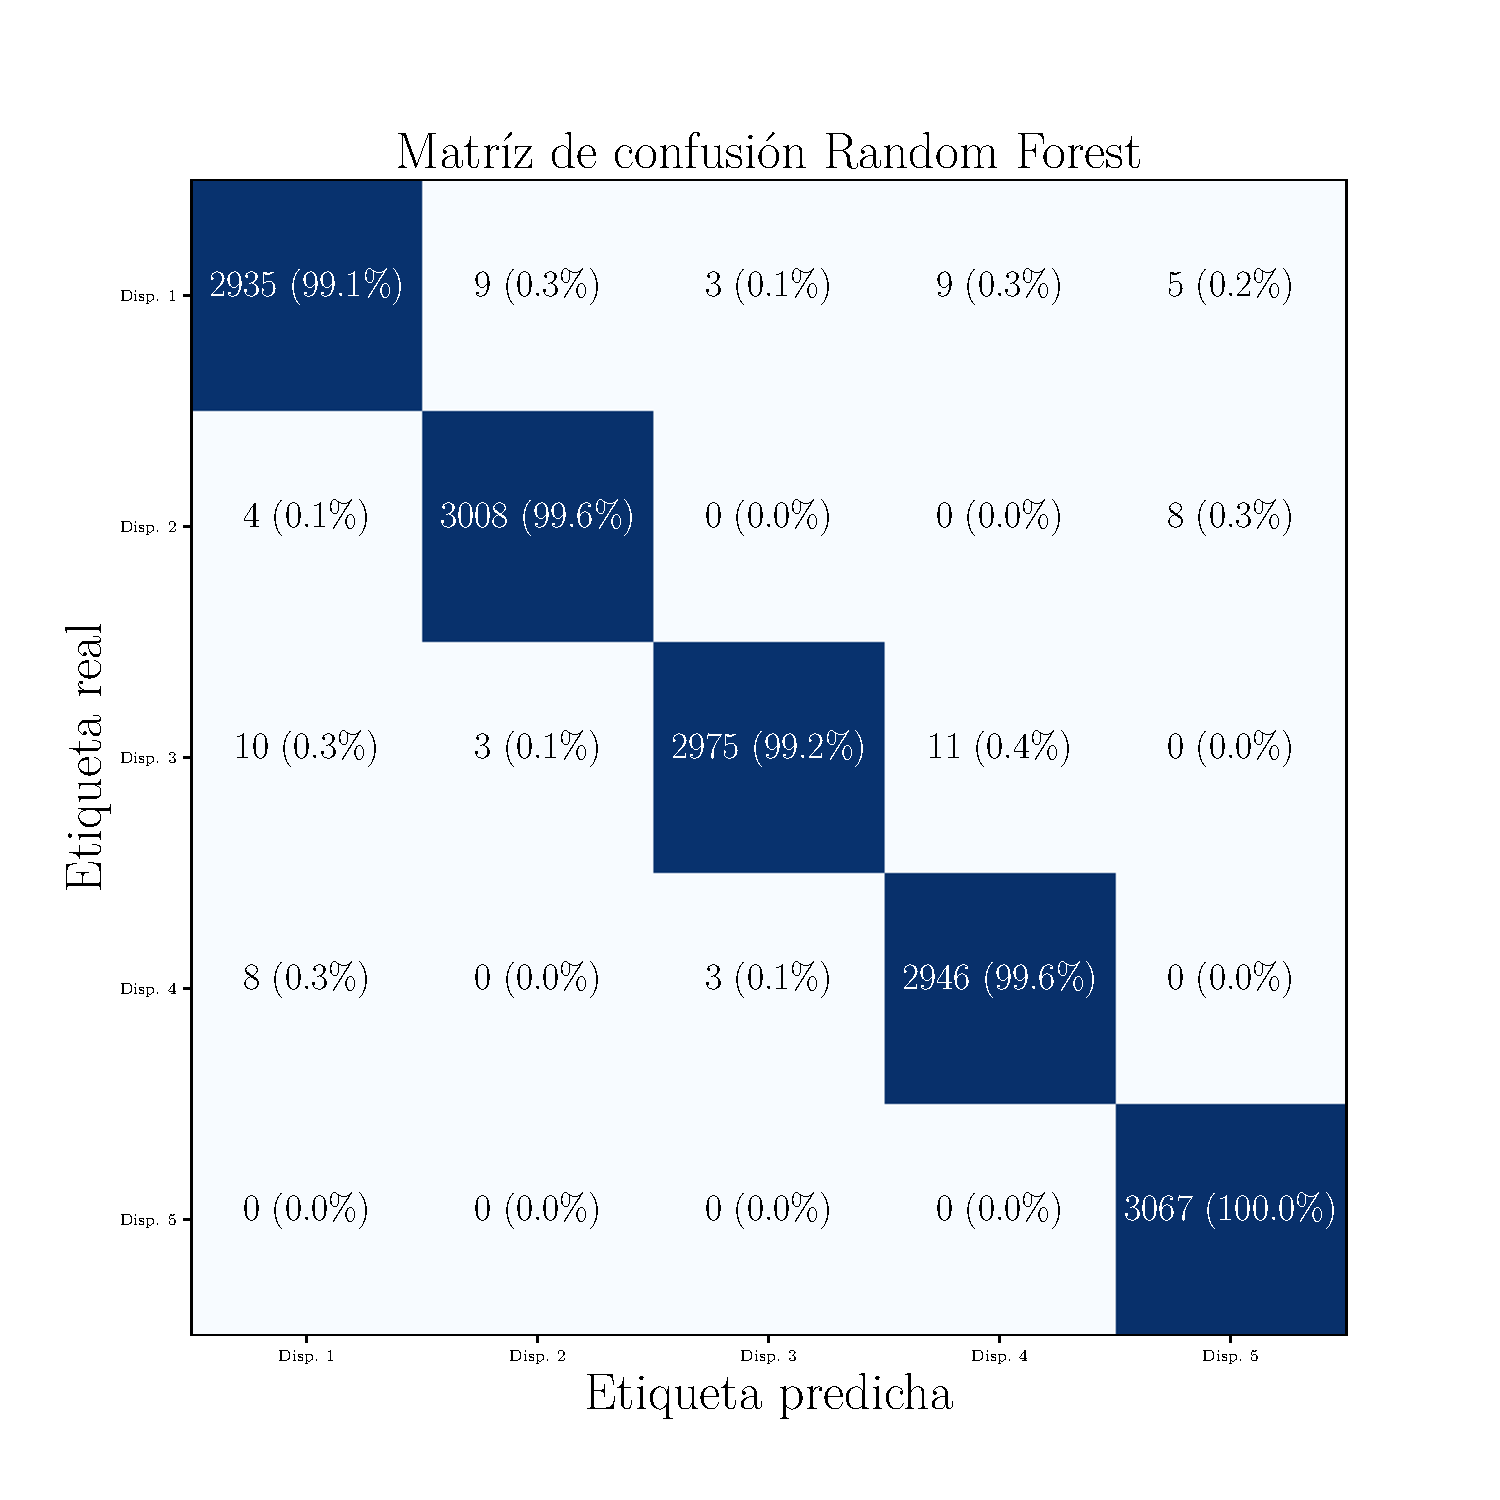
\includegraphics[width=0.4\textwidth]{../Python/plots/parallel/random_forest_matrix}} & \multirow{3}{*}[8em]{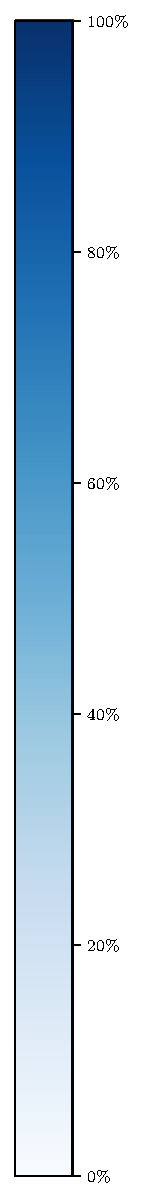
\includegraphics[scale=0.75]{../Python/plots/parallel/colorbar_matrices}} \\
        \subfloat{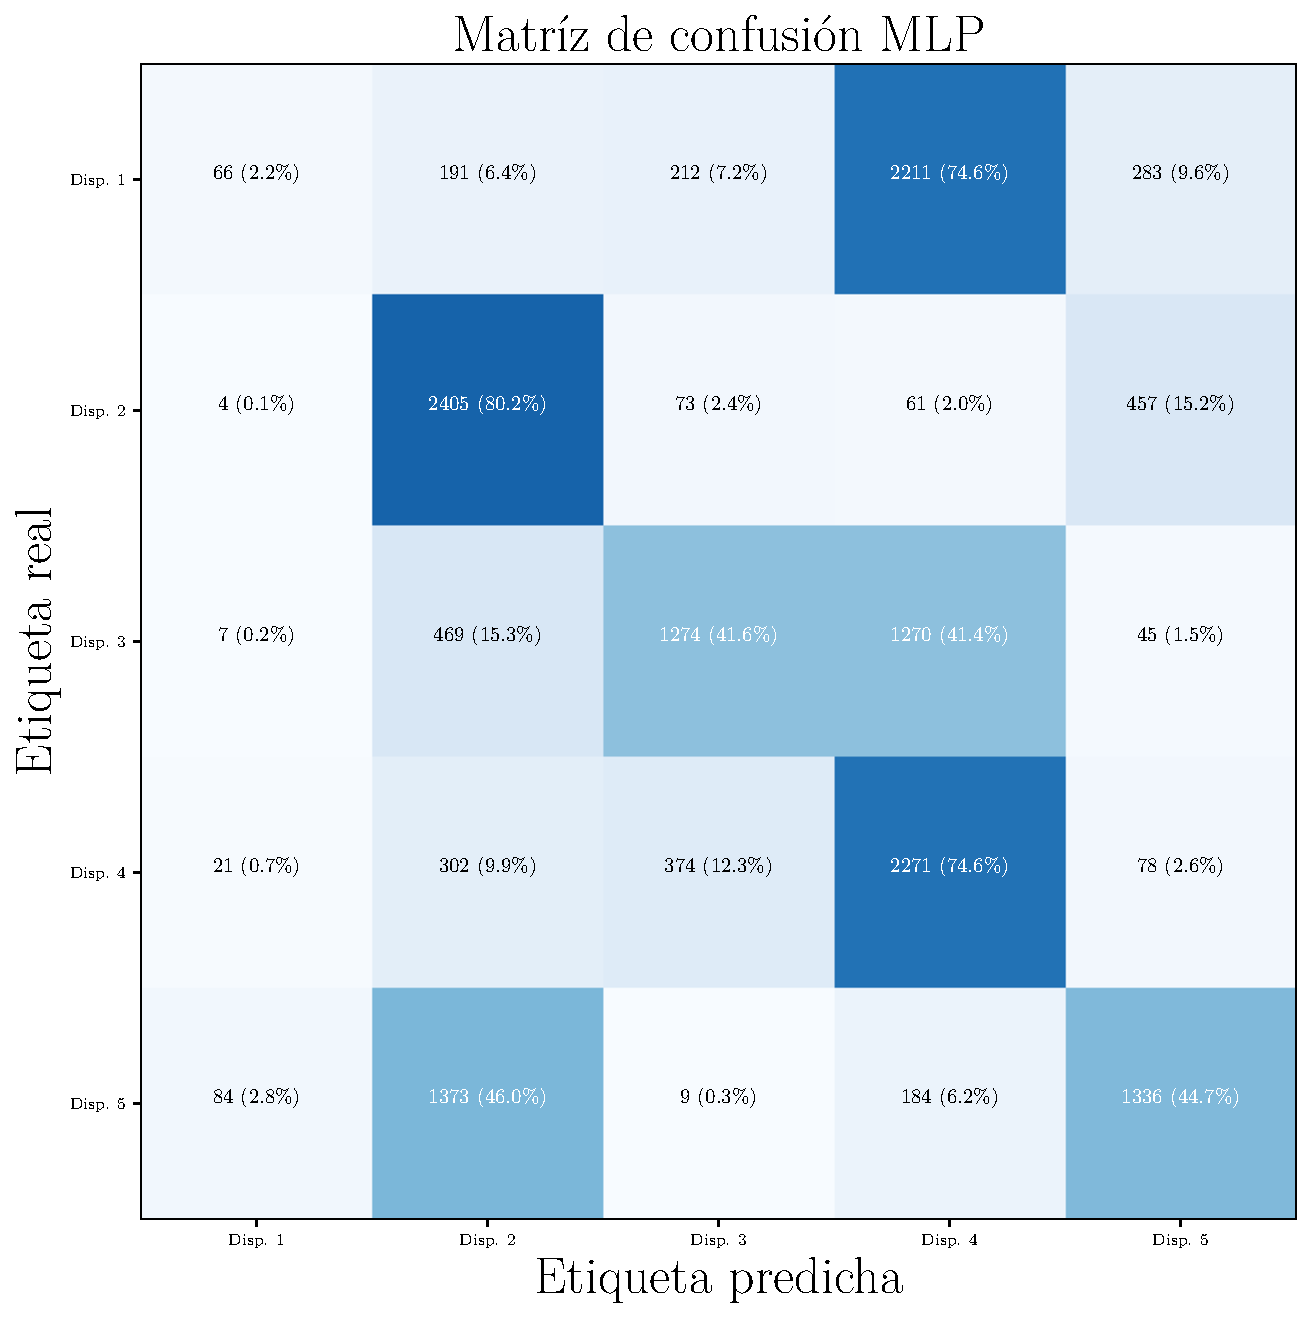
\includegraphics[width=0.4\textwidth]{../Python/plots/parallel/mlp_matrix}} & \subfloat{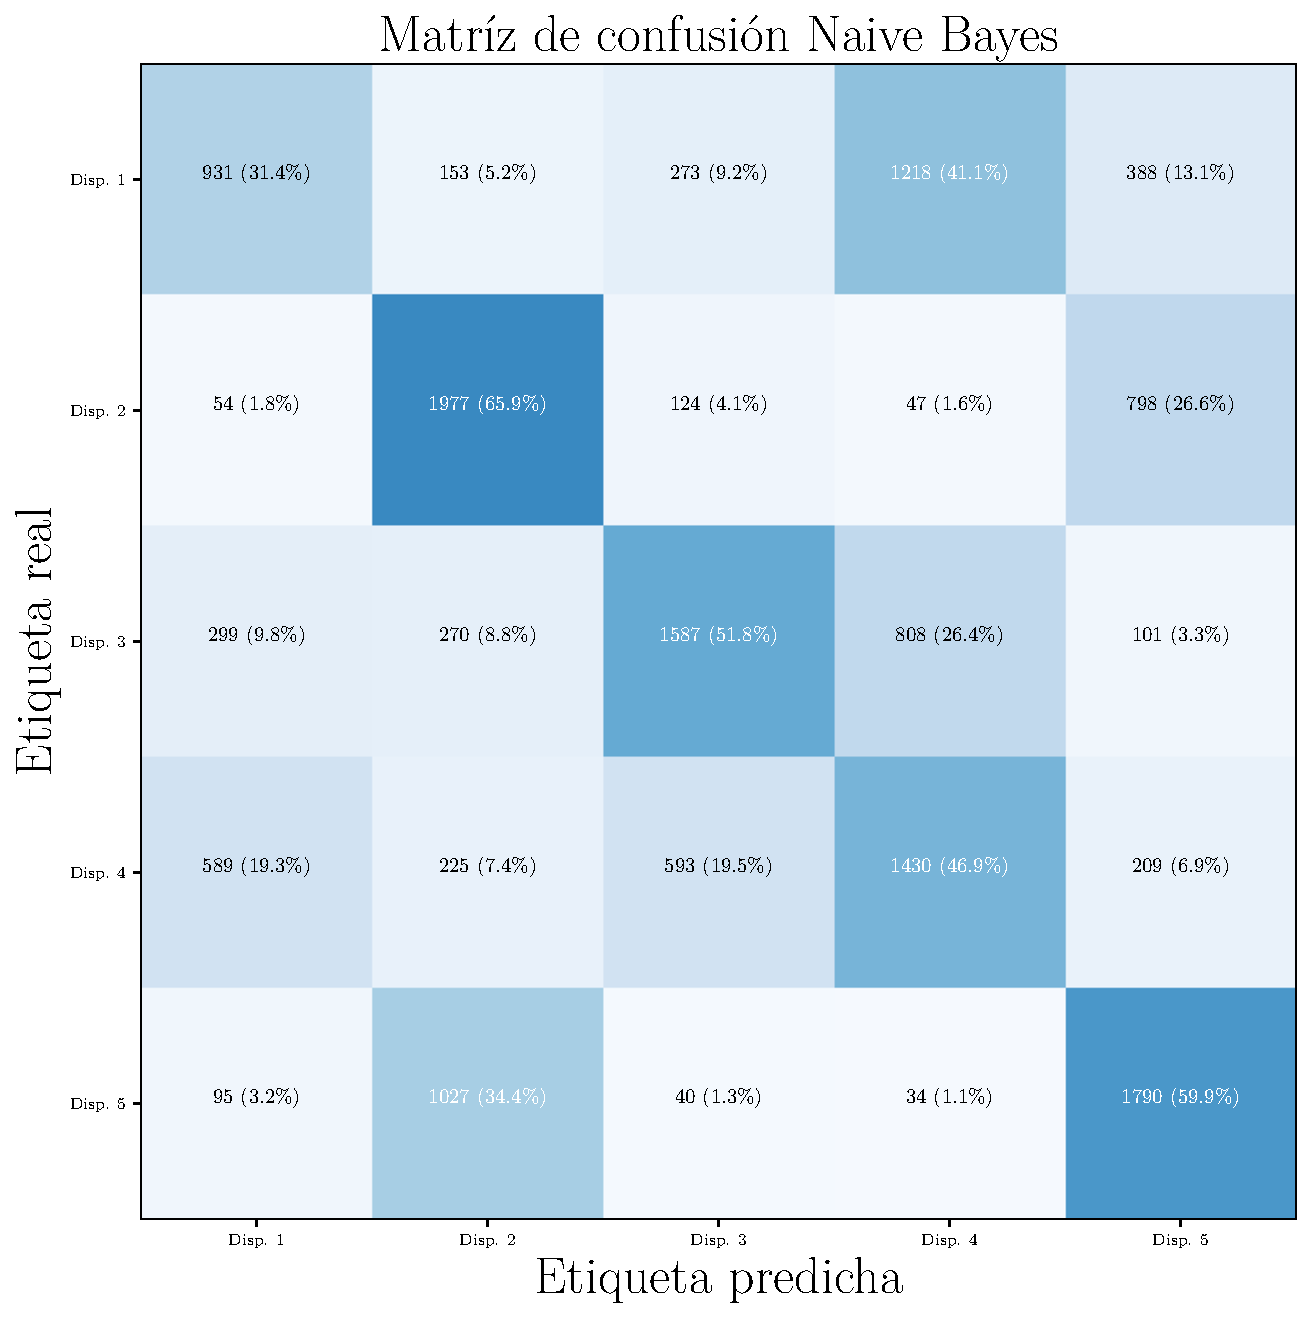
\includegraphics[width=0.4\textwidth]{../Python/plots/parallel/naive_bayes_matrix}} &  \\
        \subfloat{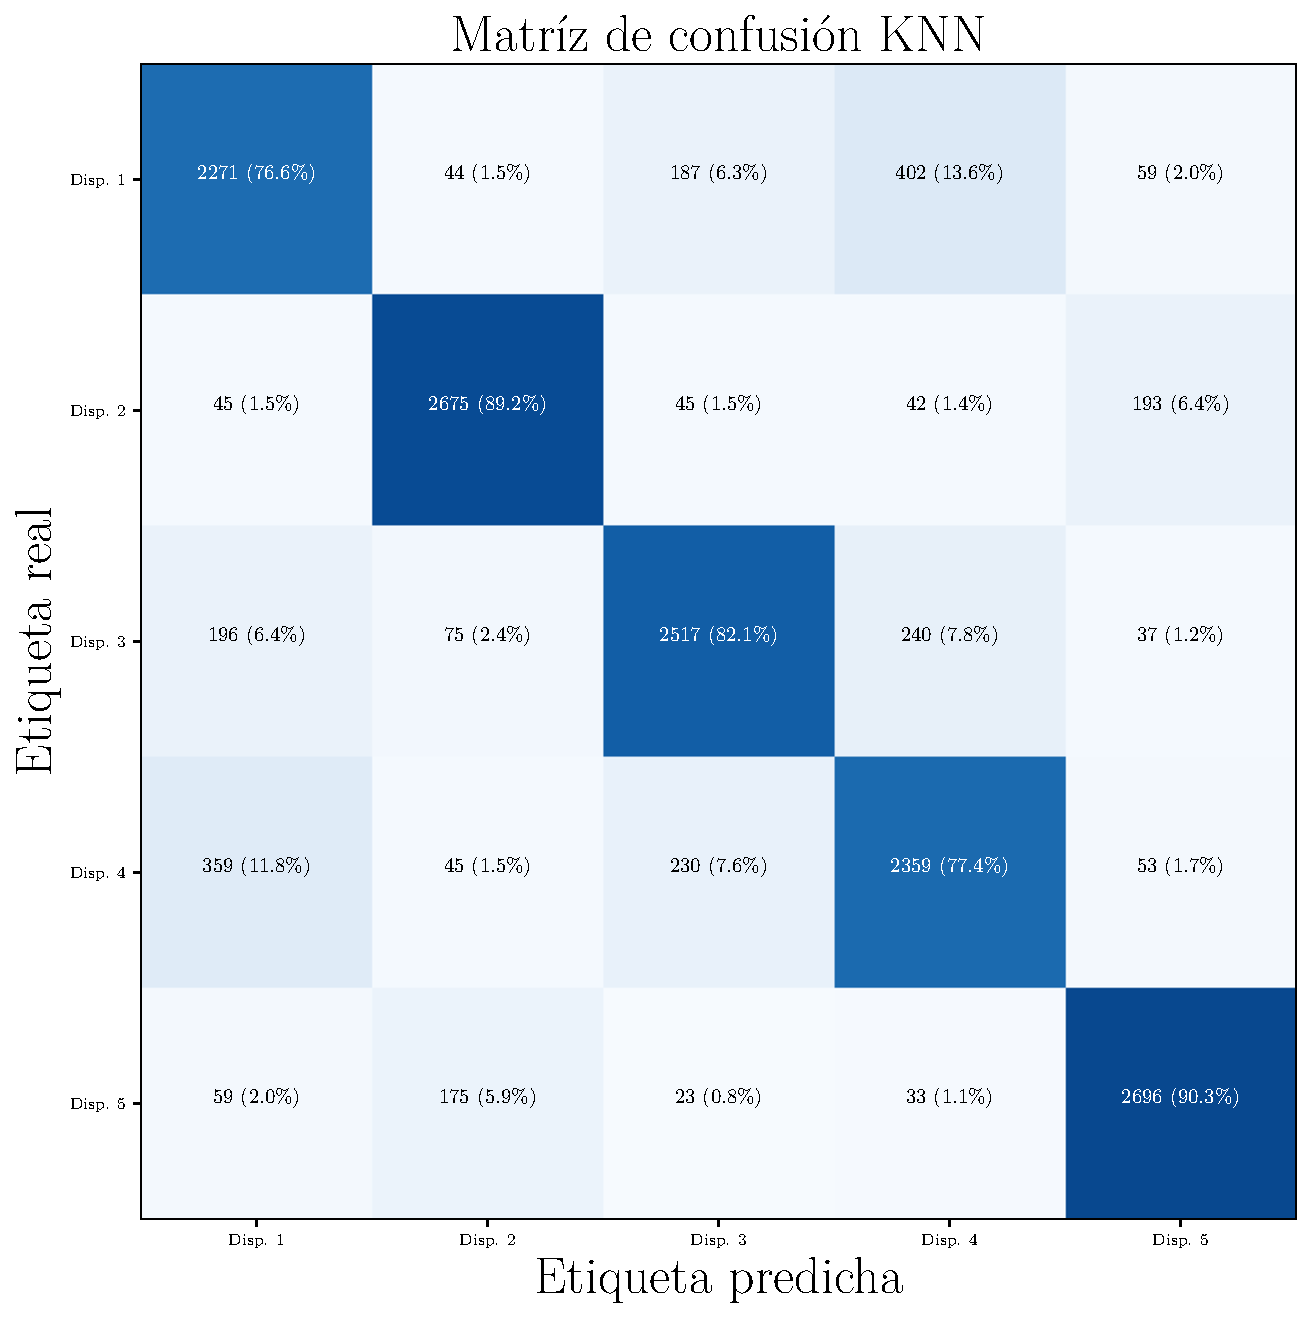
\includegraphics[width=0.4\textwidth]{../Python/plots/parallel/knn_matrix}} & \subfloat{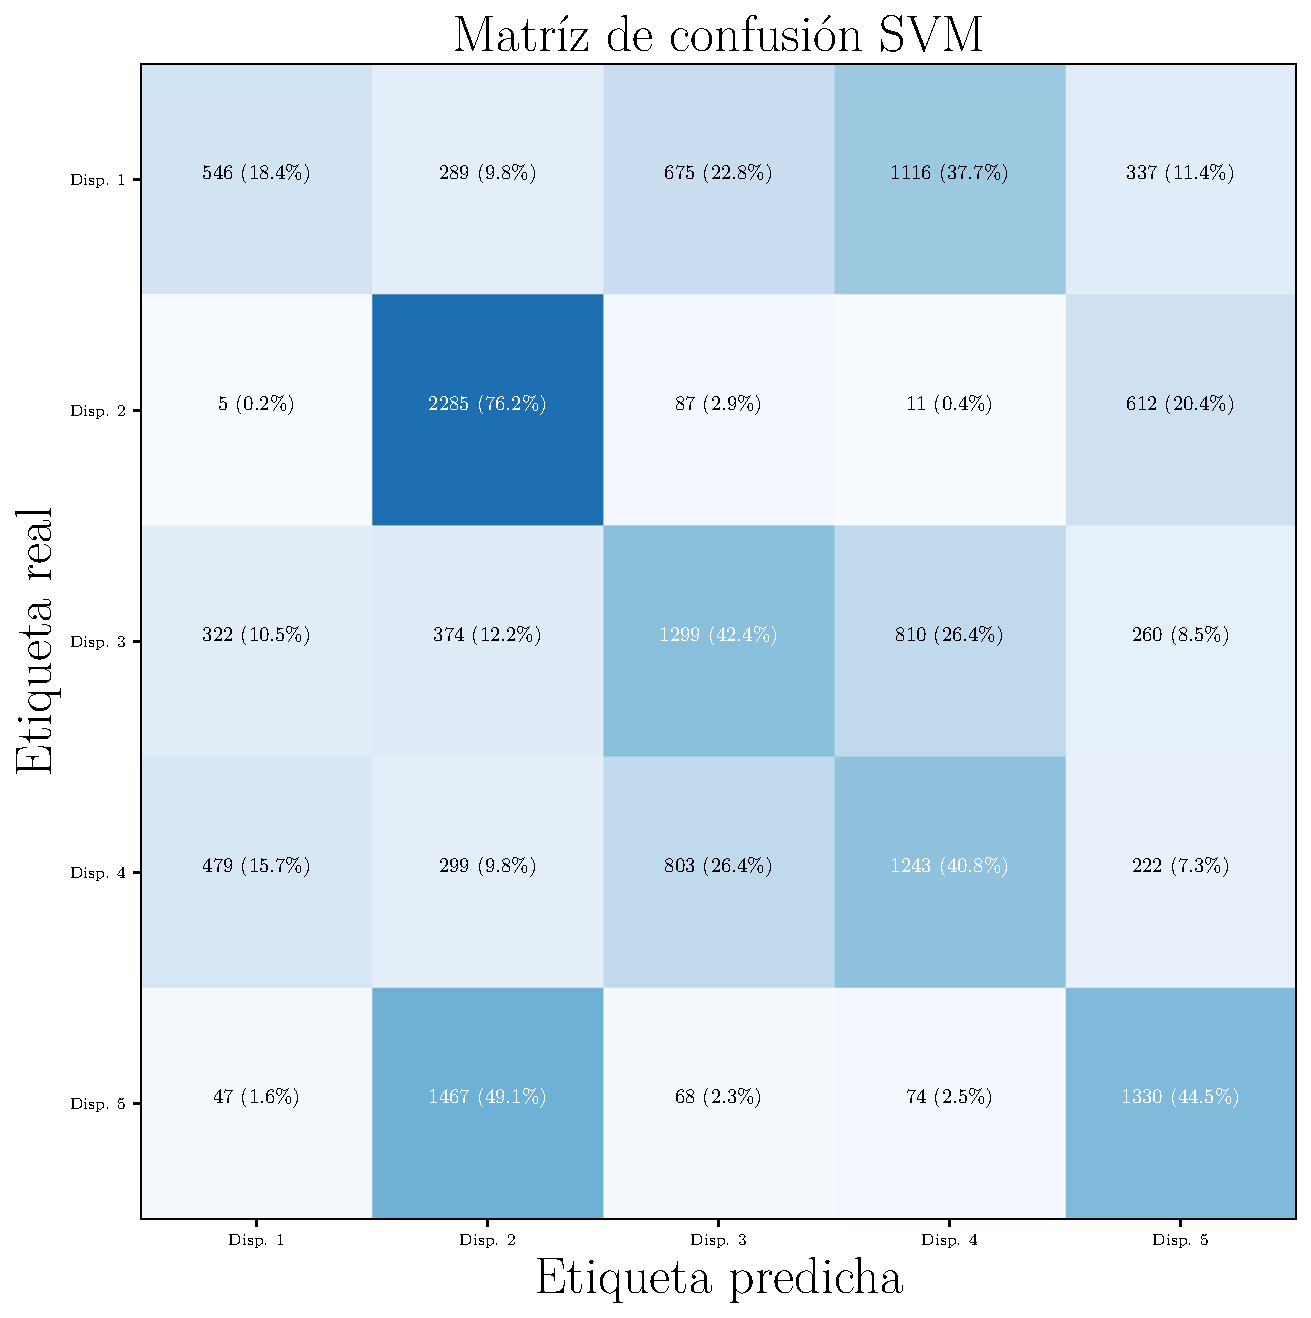
\includegraphics[width=0.4\textwidth]{../Python/plots/parallel/svm_linear_matrix}} & \\
    \end{tabular}
    \caption{Matrices de confusión con datos de la muestra paralela}
    \label{fig:confusion_matrices_parallel}
\end{figure}

Desde el punto de vista de los modelos de detección de anomalías, no se han obtenido valores de las métricas tan altas como en los algoritmos de clasificación vistos anteriormente. Se pone como ejemplo el cálculo de las métricas de Recall y TNR que se hace en función de las dos matrices de confusión, Tabla \ref{tab:ex_unsupervised_results}, que genera el par $\langle
$Dispositivo, Algoritmo$\rangle$.

En la evaluación de detectar como valores correctos los de su propio dispositivo se obtiene un Recall, usando la Fórmula \ref{eq:recall}, de 95.12\%. Este valor es obtenido mediante la matriz de confusión mostrada en la Tabla \ref{tab:iso_disp1_recall}. Por contra, en la tarea de detectar como valores anómalos los provenientes del resto de dispositivos (Tabla \ref{tab:iso_disp1_tpr}), no obtiene un valor tan elevado, tan solo un 10.36\% de TNR (Fórmula \ref{eq:tnr}).

\begin{table}[htpb!]
    \centering
    \subfloat[20\% de los datos del Disp. 1]{
    \begin{tabular}{@{}cc cc@{}}
        \multicolumn{1}{c}{} &\multicolumn{1}{c}{} &\multicolumn{2}{c}{Valor predicho} \\ 
        \cmidrule(lr){3-4}
        \multicolumn{1}{c}{} & 
        \multicolumn{1}{c}{} & 
        \multicolumn{1}{c}{Sí} & 
        \multicolumn{1}{c}{No} \\ 
        \cline{2-4}
        \multirow[c]{2}{*}{\rotatebox[origin=tr]{90}{$\underset{\text{real}}{\text{Valor}}$}}
        & Sí  & 8034 & 412 \\
        & No  & 0 & 0 \\ 
        \cline{2-4}
        \label{tab:iso_disp1_recall}
    \end{tabular}
    } \qquad
    \subfloat[20\% de los datos de todos excepto el Disp. 1]{
    \begin{tabular}{@{}cc cc@{}}
        \multicolumn{1}{c}{} &\multicolumn{1}{c}{} &\multicolumn{2}{c}{Valor predicho} \\ 
        \cmidrule(lr){3-4}
        \multicolumn{1}{c}{} & 
        \multicolumn{1}{c}{} & 
        \multicolumn{1}{c}{Sí} & 
        \multicolumn{1}{c}{No} \\ 
        \cline{2-4}
        \multirow[c]{2}{*}{\rotatebox[origin=tr]{90}{$\underset{\text{real}}{\text{Valor}}$}}
        & Sí  & 0 & 0 \\
        & No  & 29027 & 3354 \\ 
        \cline{2-4}
        \label{tab:iso_disp1_tpr}
    \end{tabular}
    }
    \caption{Matrices de confusión del Disp. 1 con el modelo de Isolation Forest}
    \label{tab:ex_unsupervised_results}
\end{table}

El resto de valores de la tabla de resultados (Tabla \ref{tab:anomaly_results}) son generados mediante el mismo procedimiento.

\begin{table}[htpb!]
    \centering
    \begin{tabular}{lcccccc}
    \toprule
     & \multicolumn{2}{c}{\texttt{Isolation Forest}} & \multicolumn{2}{c}{\texttt{Local Outlier Factor}} & \multicolumn{2}{c}{\texttt{OneClass-SVM}} \\
    \cmidrule(lr){2-3}\cmidrule(lr){4-5}\cmidrule(lr){6-7}
    & $Recall$ & $TNR$ & $Recall$ & $TNR$ & $Recall$ & $TNR$ \\
    \midrule
     Disp. 1 & 95.12\% & 10.36\% & 98.99\% & 10.68\% & 49.48\% & 58.24\% \\
     Disp. 2 & 94.98\% & 28.87\% & 98.45\% & 57.74\% & 50.90\% & 70.36\% \\
     Disp. 3 & 94.80\% & 13.90\% & 98.73\% & 13.64\% & 49.84\% & 52.65\% \\
     Disp. 4 & 95.80\% & 16.61\% & 98.88\% & 8.74\% & 50.54\% & 64.66\% \\
     Disp. 5 & 94.89\% & 46.99\% & 98.63\% & 77.98\% & 49.53\% & 94.59\% \\
    \bottomrule
\end{tabular}

    \caption{Resultados de los modelos de detección de anomalías}
    \label{tab:anomaly_results}
\end{table}

Atendiendo al resto de valores de los modelos de detección de anomalías, se puede observar en la Tabla \ref{tab:anomaly_results} que ninguno de los modelos entrenados es capaz de identificar de una forma solvente a los distintos dispositivos. El mejor entre ellos es OneClass-SVM, pero no es capaz de obtener resultados tan elevados en comparación con los modelos de clasificación.

Una vez comparados todos los modelos que han sido creados para este trabajo, se llega a la conclusión de que el mejor entre ellos es el algoritmo de clasificación Random Forest. Por ello se ha generado un modelo final con los hiperparámetros ajustados anteriormente y con la totalidad de los datos de entrenamiento. Los resultados obtenidos se pueden ver en la matriz de confusión resultante (Fig. \ref{fig:final_matrix}). Con estos resultados se tiene un valor final de Accuracy de 99.38\%, de Recall de 99.39\% y de $f$-score de 99.38\%.



\begin{figure}[H]
    \centering
    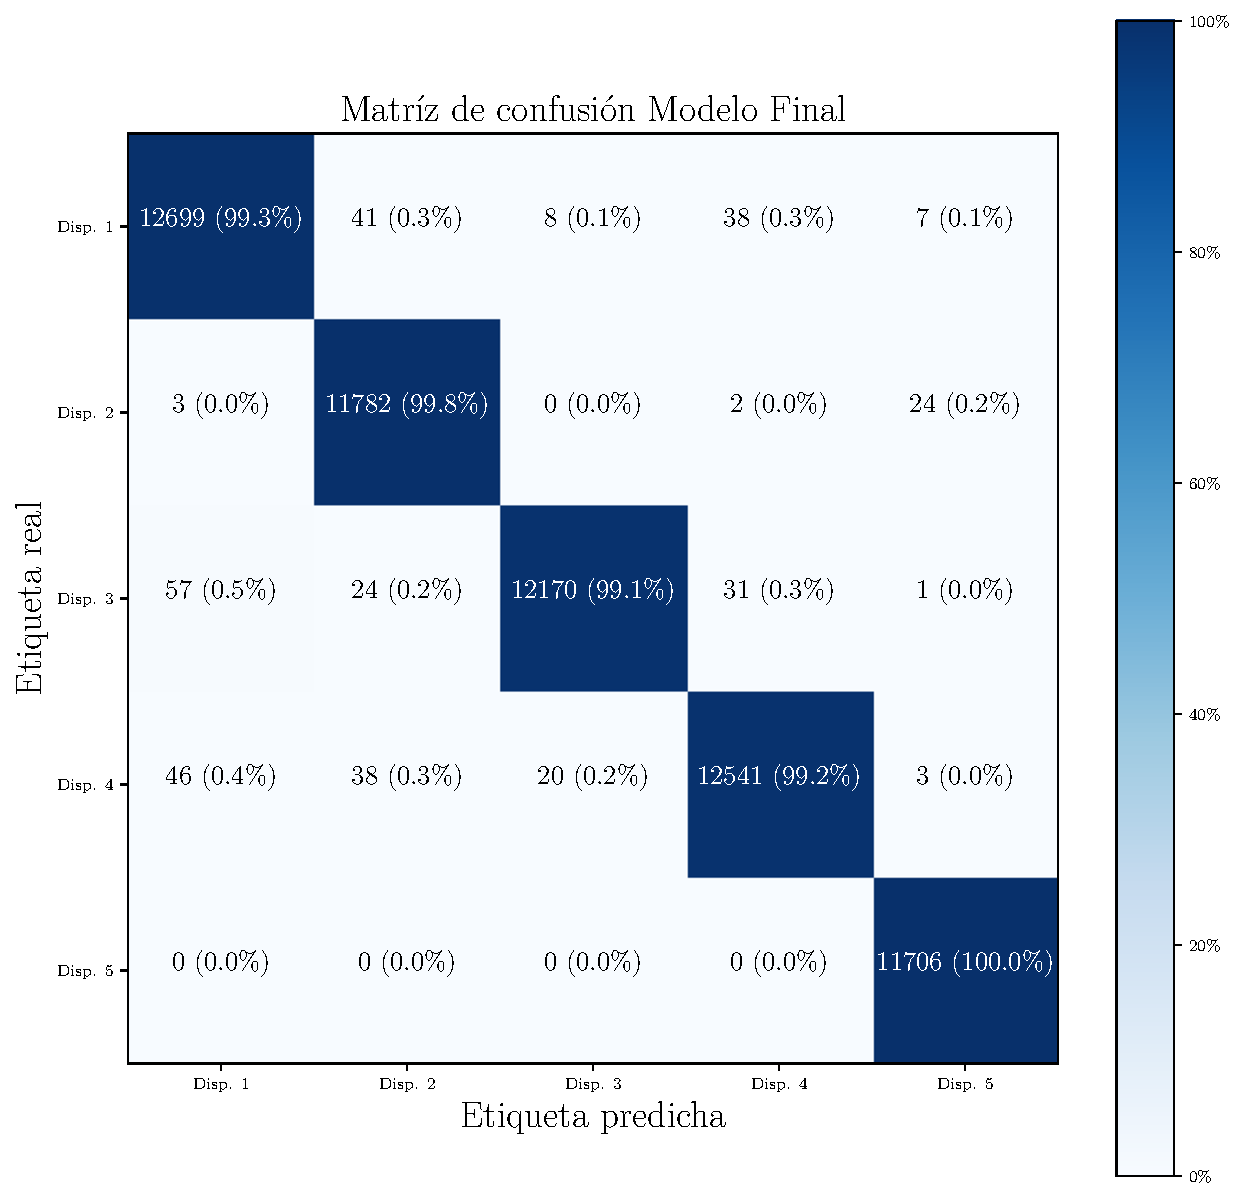
\includegraphics[scale=0.3]{../Python/plots/parallel/final_model_matrix}
    \caption{Matríz de confusión del modelo final}
    \label{fig:final_matrix}
\end{figure}
